\graphicspath{{1complete/asy/}}

\title{Math 140A - Notes}
\author{Neil Donaldson}
\date{\today}
\maketitle

\thispagestyle{empty}

\section*{Introduction}

Analysis is one of the major sub-disciplines of mathematics, concerned with continuity, limits, calculus, and accurate approximations.
\smallbreak

Analytic ideas date back thousands of years. For instance, Archimedes (c.\,287--212\,\BC) used limit-type approaches to approximate the circumference of a circle and to compute the area under a parabola.\footnote{%
	Archimedes' circle is reminiscent of Riemann sums; his parabola requires evaluation of the infinite series $\sum\limits_{n=0}^\infty \frac 1{4^n}=\frac 43$.%
}
Philosophical objections to such ideas are just as old: how can it make sense to sum infinitely many infinitesimally small quantities? This was part of a deeper debate among the ancient Greeks and other cultures: is the matter comprising the natural world \emph{atomic} (consisting of minute, discrete, indivisible objects) or \emph{continuous} (arbitrarily and infinitely divisible). Several of Zeno's famous paradoxes (5\th\,C.{}\BC) grapple with such difficulties: \emph{Achilles and the Tortoise} is essentially an argument that the infinite series $\sum\limits_{n=1}^\infty \frac 1{2^n}=\frac 12+\frac 14+\frac 18+\frac 1{16}+\cdots$ is meaningless.
\begin{center}
	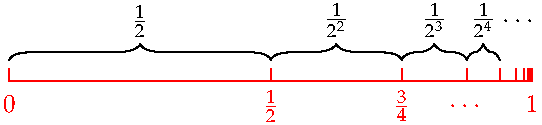
\includegraphics{zeno-jump}
\end{center}
As the picture suggests, with modern definitions it makes sense for this sum to evaluate to 1.
\smallbreak

The development of calculus by Newton, Leibniz and others in the late 1600s permitted the easy application of infinitesimal ideas to important problems in the sciences, though they did not properly address the ancient philosophical concerns. The main subject of this course (and its sequel) is the rigorous logical development of the foundations of calculus: the triumph of 18\th--19\th{} century mathematics. The critical notions of limit and continuity only became settled in during the early 1800s (courtesy of Bolzano, Cauchy, Weierstrass and others), with another 50 years passing before Riemann's thorough description of the definite integral.
\medbreak

In this course we consider sequences, limits, continuity and infinite series, with power series, differentiation and integration relegated to the sequel. We begin with something more basic: to numerically measure continuous quantities, we need to familiarize ourselves with the \emph{real numbers.} A concrete description is difficult, so we build up to it via the natural numbers and the rationals\ldots


\goodbreak

\section{Completeness}\label{sec:complete}

\subsection[The Set N of Natural Numbers]{The Set $\N$ of Natural Numbers}\label{sec:natural}

You've been using the natural numbers $\N=\{1,2,3,4,5,\ldots\}$ since you first learned to count. In mathematics, these must be \emph{axiomatically} described. Here is one approach.

\begin{axioms}{Peano}{Peano}
	The natural numbers are a set $\N$ satisfying the following properties:
	\begin{enumerate}
	  \item (Non-emptiness)\lstsp $\N$ is non-empty.
		\item (Successor function)\lstsp There exists a function $f:\N\to\N$. This is usually denoted `$+1$' so that we may write,
		\[
			n\in\N\implies n+1\in\N
		\]
		\item (Initial element)\lstsp The successor function $f$ is \emph{not surjective.} Otherwise said, there is an element $1\not\in\operatorname{range}f$ which is not the successor of any element.\footnotemark
		\item (Unique predecessor/order)\lstsp $f$ is \emph{injective.} Otherwise said,
		\[
			m+1=n+1\implies m=n
		\]
		\item (Induction)\lstsp Suppose $A\subseteq\N$ is a subset satisfying
		\begin{enumerate}
		  \item $1\in A$,\qquad\qquad
		  (b)\ \ $n\in A\Longrightarrow n+1\in A$.
		\end{enumerate}
		Then $A=\N$.
	\end{enumerate}
\end{axioms}

\footnotetext{%
	By convention, the first natural number is 1; we could use 0, $x$, $\alpha$, or any symbol you wish!%
}

Axioms 1--4 state that $\N$ is defined by repeatedly adding 1 to the initial element; for instance
\[
	3:=f\bigl(f(1)\bigr)=f(1+1)=(1+1)+1
\]
Parts (a) and (b) of axiom 5 are the familiar \emph{base case} and \emph{induction step} a standard induction: let $P_n$ be the proposition `$n\in A$' to recover the usual form of the \emph{Principle of Mathematical Induction.}

\begin{example}{}{}
	Prove that $7^n-4^n$ is divisible by 3 for all $n\in\N$.
	\smallbreak
	Let $A$ be the set of natural numbers for which $7^n-4^n$ is divisible by 3. It is required to prove that $A=\N$.
	\begin{enumeratea}
	  \item If $n=1$, then $7^1-4^1=3$, whence $1\in A$.
	  \item Suppose $n\in A$. Then $7^n-4^n=3\lambda$ for some $\lambda\in\N$. But then
		\begin{align*}
			7^{n+1}-4^{n+1}&=7\cdot 7^n-4^{n+1}=7(3\lambda+4^n)-4^{n+1}=3\cdot 7\lambda+(7-4)\cdot 4^n\\
			&=3\bigl(7\lambda+4^n\bigr)
		\end{align*}
	is divisible by 3. It follows that $n+1\in A$.
	\end{enumeratea}
	Appealing to axiom 5, we see that $A=\N$, hence result.
\end{example}

\goodbreak

\boldinline{What about the integers?}

The integers satisfy only axioms 1, 2 and 4. For instance:
\begin{itemize}
  \item[$\not\!3$.] The function $f:\Z\to\Z:n\mapsto n+1$ is surjective (indeed bijective/invertible). The `initial element' $1\in\N$ is the successor of $0\in\Z$.  
\end{itemize}

Reversing this observation provides an explicit construction of $\Z$ from $\N$: simply extend the successor function $f$ so that every element has a unique predecessor: 0 is the unique predecessor of 1, $-1$ the unique predecessor of 0, etc. In essence we are forcing $f(n)=n+1$ to be bijective!


\goodbreak


\begin{exercises}{}{}
	\emph{Key concepts/results:\quad Peano's Axioms,\quad Induction}\smallbreak
	
	Most of these exercises are to refresh your memory of induction. Use either the language of Peano's axiom 5, or the (possibly) more familiar base-case/induction-step formulation.	
	\begin{enumerate}
	  \item%[1.]
	  Prove that $1^2+2^2+\cdots+n^2=\frac 16n(n+1)(2n+1)$ for all natural numbers $n$.
	  
	  
	  \item%[2.]
	  Prove that $3+11+\cdots+(8n-5)=4n^2-n$ for all $n\in\N$.
	
	
	  \item%[4.]
	  \begin{enumerate}
	  	\item Guess a formula for $1+3+\cdots+(2n-1)$ by evaluating the sum for $n=1,2,3$, and 4.\par
	  	(\emph{For $n=1$ the sum is simply 1})
	  
	  	\item Prove your formula using mathematical induction.
	  \end{enumerate}
	  
	  
	  \item%[6.]
	  Prove that $11^n-4^n$ is divisible by 7 for all $n\in\N$.
	  
	  
	  \item%[8.]
	  The principle of mathematical induction can be extended as follows. A list $P_m,P_{m+1},\ldots$ of propositions is true provided (i) $P_m$ is true, (ii) $P_{n+1}$ is true whenever $P_n$ is true and $n\ge m$.
	  \begin{enumerate}
	  	\item Prove that $n^2>n+1$ for all integers $n\ge 2$.
	  	\item Prove that $n!>n^2$ for all integers $n\ge 4$.\hfill
	  	(\emph{recall that $n!=n(n-1)\cdots 2\cdot 1$})
	  \end{enumerate}
	  
	  
	  \item%[10.]
	  Prove $(2n+1)+(2n+3)+(2n+5)+\cdots+(4n-1)=3n^2$ for all $n\in\N$.
	  
	  
	  \item%[11.]
	  For each $n\in\N$, let $P_n$ denote the assertion ``$n^2+5n+1$ is an even integer''.
	  \begin{enumerate}
	  	\item Prove that $P_{n+1}$ is true whenever $P_n$ is true.
	  	\item For which $n$ is $P_n$ actually true? What is the moral of this exercise?
	  \end{enumerate}
	  
	  
	  \item%[12.]
		For $n\in\N$, let $n!$ denote the factorial function ($0!=1$) and define the binomial coefficient
	  \[
	  	\binom nk=\frac{n!}{k!(n-k)!}\quad\text{for}\quad\ k=0,1,\ldots,n
	  \]
	  The \emph{binomial theorem} asserts that, for all $n\in\N$,
	  \[
	  	(a+b)^n =\sum_{k=0}^n\binom nk a^{n-k}b^k
	  	=a^n+na^{n-1}b+\frac{n(n-1)}2a^{n-2}b^2+\cdots+nab^{n-1}+b^n
	  \]
	  \begin{enumerate}
	  	%\item Verify the binomial theorem for $n=1,2$, and 3.
	  	\item Show that $\binom nk+\binom n{k-1}=\binom{n+1}k$ for $k=1,2,\ldots,n$.
	  	\item Prove the binomial theorem by induction.
	  \end{enumerate}
	
	
	  \item Show that Peano's induction axiom is \emph{false} for the set of integers $\Z$ by exhibiting a \emph{proper subset} $A\subset\Z$ which satisfies conditions (a) and (b).
	  
	  
	  \item Consider $\Z_3=\{0,1,2\}$ under addition modulo 3. That is,
	  \[
	  	0+1=1,\quad 1+1=2,\quad 2+1=0
	  \]
	  Which of Peano's axioms are satisfied?
	\end{enumerate}
\end{exercises}


\clearpage



\subsection[The Set Q of Rational Numbers]{The Set $\Q$ of Rational Numbers}\label{sec:Q}

The rational numbers may be defined in several ways. For instance, we could consider the set of relatively prime ordered pairs
\[
	\Q=\bigl\{(p,q):p\in\Z,\ q\in\N,\, \gcd(p,q)=1\bigr\}\subseteq\Z\times\N
\]
Things seem more familiar if we write $\frac pq$ instead of $(p,q)$ and adopt the convention that $\frac{\lambda p}{\lambda q}=\frac pq$ for any non-zero $\lambda\in\Z$. The usual operations ($+,\cdot$, etc.) are easily defined, consistently with those for the integers (Exercise \ref{exs:ratnumber+x}).
\smallbreak

An alternative approach involves equations. Each \emph{linear equation} $qx-p=0$ where $p,q\in\Z$ and $q\neq 0$ corresponds to a rational number. For example
\[
	13x+27=0\leftrightsquigarrow x=-\frac{27}{13}
\]
Of course the equation $26x+54=0$ \emph{also} corresponds to the same rational number!
\medbreak

Extending this process naturally leads us to consider higher degree polynomials.

\begin{defn}{}{}
	A number $x$ is \emph{algebraic} if it satisfies an equation of the form\footnotemark
	\[
		a_nx^n+a_{n-1}x^{n-1}+\cdots+a_1x+a_0=0\tag*{$(\ast)$}
	\]
	for some integers $a_0,\ldots,a_n$.
\end{defn}

\footnotetext{%
	You should be alarmed by this! We seem to have given up \emph{constructing} new numbers and instead are merely \emph{describing} their properties. No matter, a construction of the real numbers will come later.%
}

\begin{examples}{}{}
	\exstart $\sqrt 2$ is algebraic since it satisfies the equation $x^2-2=0$.

	\begin{enumerate}\setcounter{enumi}{1}
	  \item $x=\sqrt[5]{7+\sqrt 3}$ is also algebraic:
	  \[
	  	x^5-7=\sqrt 3\implies (x^5-7)^2=3\implies x^{10}-14x^5+46=0
	  \]
	\end{enumerate}
\end{examples}


The next result is helpful for deciding whether a given number is rational and can assist with factorizing polynomials.

\begin{thm}{Rational Roots}{ratroots}
	Suppose $a_0,\ldots,a_n\in\Z$ and that $x\in\Q$ satisfies $(\ast)$. If $x=\frac pq$ is rational, written in lowest terms, then $p\mid a_0$ and $q\mid a_n$.
\end{thm}


\begin{proof}
	Substitute $x=\frac pq$ into the polynomial equation and multiply through by $q^n$ to see that
	\[
		a_np^n+a_{n-1}p^{n-1}q+\cdots+a_1pq^{n-1}+a_0q^n=0
	\]
	This is an equation \emph{in integers.} All terms except the last contain a factor of $p$, whence $p\mid a_0q^n$. Since $\gcd(p,q)=1$, it follows that $p\mid a_0$. The result for $q$ is almost identical: all but the first term above has a factor of $q$.
\end{proof}


\goodbreak


\begin{examples}{}{}
	\exstart We prove that $\sqrt 2$ is irrational.	Plainly $x=\sqrt 2$ satisfies the polynomial equation $x^2-2=0$. If $\sqrt 2=\frac pq$ were rational in lowest terms, then the rational roots theorem forces
	\[
		p\mid 2\quad\text{and}\quad q\mid 1\implies \sqrt 2\in\{\pm 1,\pm 2\}
	\]
	Since none of the values $\pm 1,\pm 2$ satisfy $x^2-2=0$, we have a contradiction.

	\begin{enumerate}\setcounter{enumi}{1}
		\item $y=(\sqrt 3-1)^{1/3}$ satisfies $(y^3+1)^2=3$, whence $y^6+2y^3-2=0$. If $y=\frac pq$ were rational in lowest terms, then $p\mid 2$ and $q\mid 1$, whence $y=\pm 1,\pm 2$; none of which satisfy the polynomial.
		
		\item $z=\left(\frac{4+\sqrt 3}{5}\right)^{1/2}$ satisfies $5z^2-4=\sqrt 3$, from which $25z^4-40z^2+13=0$. If $z=\frac pq$ were rational in lowest terms, then $p\mid 13$ and $q\mid 25$. There are twelve possibilities: it is tedious to check, but none satisfy the required polynomial,
		\[
			z=\pm 1,\ \pm 13,\ \pm\tfrac 15,\ \pm\tfrac{13}5,\ \pm\tfrac 1{25},\ \pm\tfrac{13}{25}
		\]
		In this case it is easier to bypass the theorem: if $z\in\Q$ then $\sqrt 3=5z^2-4$ would also be rational!
		
		\item We use the theorem to factorize the polynomial $3x^3+x^2+x-2=0$. If $x=\frac pq$ is a rational root, then $p\mid 2$ and $q\mid 3$ give several possibilities:
		\[
			x\in\left\{\pm 1,\pm 2,\pm\tfrac 13,\pm\tfrac 23\right\}
		\]
		It doesn't take long to check that $x=\frac 23$ is the only rational root. A factor of $3x-2$ may be extracted by long division to obtain
		\[
			3x^3+x^2+x-2=(3x-2)(x^2+x+1)
		\]
		The quadratic has no real roots: absent complex numbers, the factorization is complete.
	\end{enumerate}
\end{examples}

It is far from clear that non-algebraic (\emph{transcendental}) numbers exist: $e$ and $\pi$ are the most famous. These satisfy no polynomial equation with integer coefficients, though demonstrating such is tricky.


\begin{exercises}{}
	\emph{Key concepts:\quad Algebraic Numbers,\quad Rational Roots Theorem/Testing for Irrationality}

	\begin{enumerate}
	  \item Describe all linear equations corresponding to the rational number $\frac{101}{29}$.
	  
	  \item %[1.]
	  Show that $\sqrt 3$, $\sqrt 5$ and $\sqrt{24}$ are not rational numbers: what are the relevant polynomials?
	  
	  
	  \item %[2.]* 
	  Show that $2^{1/3}$ and $13^{1/4}$ are not rational numbers.
	
	
	  \item%[3.]+[5.]
	  Show that $(2+\sqrt 2)^{1/2}$ and $(5-\sqrt 3)^{1/3}$ are irrational.
	  
	  
	%   \item%[4.]* 
	%   Show that $(5-\sqrt 3)^{1/3}$ is not rational.
	  
	  
	  %\item%[5.] 
	  %Show that $(3+\sqrt 2)^{2/3}$ is not rational.
	  
	  
	  \item%[6.]* 
	  Explain why $4-7b^2$ must be rational if $b$ is rational.
	  
	  
	  \item\label{exs:ratnumber+x} Given rational numbers $(p,q)$, $(r,s)$ as ordered pairs, what are $(p,q)+(r,s)$ and $(p,q)\cdot(r,s)$?
	  
	  
	  \item Let $n\in\N$. Use the rational roots theorem to prove that $\sqrt n\in\Q\iff \sqrt n\in\N$.
	  
	  
	  \item In the proof of the rational roots theorem, explain why the condition $\gcd(p,q)=1$ allows us to conclude that $p\mid a_0q^n\Longrightarrow p\mid a_0$
	\end{enumerate}
\end{exercises}


\clearpage



\subsection{Ordered Fields}

We have thus far formally constructed the natural numbers and used them to build the integers and rational numbers. It is a significantly greater challenge to \emph{construct} the real numbers. We start by thinking about ordered fields, of which both $\Q$ and $\R$ are examples.

\begin{axioms}{}{field}
	A \emph{field} $\F$ is a set with two binary operations $+,\cdot$ which satisfy (for all $a,b,c\in\F$),\footnotemark
	\[
		\def\arraystretch{1.3}
		\begin{array}{@{}l||l|l}
			%\hline
			&\multicolumn{1}{c|}{\text{Addition}}
			&
			\multicolumn{1}{c}{\text{Multiplication}}\\\hline\hline
			\text{Closure}&a+b\in\F &ab\in\F\\\hline
			\text{Associativity}&a+(b+c)=(a+b)+c &a(bc)=(ab)c\\\hline
			\text{Commutativity}&a+b=b+a &ab=ba\\\hline
			\text{Identity}&\exists 0\in\F\text{ such that }a+0=a &\exists 1\in\F \text{ such that }a\cdot 1=a\\\hline
			\text{Inverse}&\exists -a\in\F \text{ such that }a+(-a)=0 &\text{If }a\neq 0,\ \exists a^{-1}\in\F\text{ such that }aa^{-1}=1\\\hline\hline
			\text{Distributivity}&\multicolumn{2}{|l}{a(b+c)=ab+ac}%\\\hline
		\end{array}
	\]
	A field $\F$ is \emph{ordered} if we also have a binary relation $\le$ which satisfies (again for all $a,b,c\in\F$):
	\[
		\def\arraystretch{1.3}
		\begin{array}{@{}ll}
			\text{O1}&a\le b\text{ or }b\le a\\
			\text{O2}&a\le b\text{ and }b\le a\implies a=b\\
			\text{O3}&a\le b\text{ and }b\le c\implies a\le c\\
			\text{O4}&a\le b\implies a+c\le b+c\\
			\text{O5}&a\le b\text{ and }0\le c\implies ac\le bc
		\end{array}
	\]
\end{axioms}

\footnotetext{%
	Write multiplication $\cdot$ as juxtaposition unless necessary, and use the common shorthand $a^2=a\cdot a$. The field axioms are very easy to remember if you know some abstract algebra:
	\begin{itemize}
  	\item The addition axioms say that $\bigl(\F,+\bigr)$ is an abelian group.
  	\item The multiplication axioms say that $\bigl(\F\setminus\{0\},\cdot\bigr)$ is an abelian group.
  	\item The distributive axiom describes how addition and multiplication interact.
	\end{itemize}%
}

For an ordered field, the symbol $<$ is used in the usual manner: $x<y\iff x\le y$ and $x\neq y$.
\smallbreak

As with Peano's axioms for the natural numbers, these are not worth memorizing. Instead you should quickly check that you believe all of them for your current understanding of the real numbers; you can't \emph{prove} anything since the real numbers are yet to be defined!
\smallbreak


\begin{example}{}{qordered}
	It is worth considering the rational numbers in a little more detail. These inherit a natural ordering from $\Z$ and $\N$:
	\[
		\frac pq\le\frac rs\iff ps\le qr \tag{remember that $q,s>0$}
	\]
  It is now possible, though tedious, to \emph{prove} that each of the axioms of an ordered field holds for $\Q$, using only basic facts about multiplication, addition and ordering \emph{within the integers.} For instance,
  \begin{description}
		\item[\normalfont\emph{Commutativity of Multiplication}] Given $a=\frac pq$ and $b=\frac st$ rational, we have
		\[
			ab=\frac{ps}{qt}=\frac{sp}{tq}=ba
		\]
		since multiplication of integers (numerator and denominator) is commutative.
		\item[\normalfont O3] Suppose $a\le b$ and $b\le c$. Write $a=\frac pq$, $b=\frac rs$ and $c=\frac tu$ where all three denominators are positive. By assumption,
		\begin{align*}
			ps\le qr\ \text{ and }\ ru\le st &\implies ps u\le qr u\le qs t\\
			&\implies pu\le qt \tag{divide by $s\neq 0$}\\
			&\implies a=\frac pq\le\frac tu= c
		\end{align*}
	\end{description}
\end{example}


\boldsubsubsection{Basic Results about ordered fields}

As with the axioms of an ordered field, these are not worth memorizing.

\begin{thm}{}{orderedfprops}
	Let $\F$ be a ordered field with at least two elements $0\neq 1$. Then:
	\[
		\def\arraystretch{1.3}
		\begin{array}{@{}rl@{\qquad\quad}rl}
	  	1.&a+c=b+c\implies a=b &2.&a\cdot 0=0\\
	  	3.&(-a)b=-(ab)&4.&(-a)(-b)=ab\\
	  	5.&ac=bc \text{ and } c\neq 0\implies a=b &6.&ab=0\implies a=0 \text{ or }b=0\\
	  	7.&a\le b\implies -b\le -a &8.&a\le b\text{ and }c\le 0\implies bc\le ac\\
	  	9.&0\le a\text{ and }0\le b\implies 0\le ab&10.&0\le a^2\\
	  	11.&0<1&12.&0<a\implies 0<a^{-1}\\
	  	13.&0<a<b\implies 0<b^{-1}<a^{-1}&&
		\end{array}
	\]
\end{thm}

All these statements should be intuitive for the fields $\Q$ and $\R$. Try proving a few using only the axioms; they are most easily done in the order presented. For instance, part 2 might be proved as follows:
\begin{align*}
	&a\cdot 0+0=a\cdot 0=a\cdot(0+0)=a\cdot 0+a\cdot 0 \tag{additive identity/distibutive axioms}\\
	\implies &0=a\cdot 0 \tag{part 1}
\end{align*}

We finish with a final useful ingredient.

\begin{defn}{}{}
	In an ordered field $\F$, the \emph{absolute value} of an element $a$ is
	\[
		\nm a:=
		\begin{cases}
			a&\text{if }a\ge 0\\
			-a&\text{if }a<0
		\end{cases}
	\]
\end{defn}

\begin{thm}{}{}
	In any ordered field:
	\begin{enumerate}
	\item $\nm a\ge 0$
	\item $\nm{ab}=\nm a\cdot \nm b$
	\item $\nm{a+b}\le \nm a+\nm b$ \lstsp ($\triangle$-inequality)
	\item $\nm{a-b}\ge \nm{\nm a-\nm b}$ \lstsp (reverse/extended $\triangle$-inequality)
	\end{enumerate}
\end{thm}

All parts are straightforward if you consider the $\pm$-cases separately for $a,b$.


\begin{exercises}{}{}
	\emph{Key concepts:\quad Ordered Field ($\Q$ an example arising naturally from $\Z$),\quad $\triangle$-inequality}
	
	\begin{enumerate}
	  \item%[1.]
	  Which of the axioms of an ordered field fail for $\N$? For $\Z$?
	  
	  \item%[4.]
	  Prove parts 11 and 13 of Theorem \ref{thm:orderedfprops}.\par
	  (\emph{Hint: You can use any of the parts that come before\ldots})
	
	
	  \item%[6.]
	  \begin{enumerate}
	  	\item Prove that $\nm{a+b+c}\le \nm a+\nm b+\nm c$ for all $a,b,c\in\R$.\par
	  	(\emph{Hint: Apply the triangle inequality twice. Don't consider eight separate cases!})
	  	\item For any $a_1,\ldots,a_n\in\R$, use induction to prove
	  	\[
	  		\nm{a_1+a_2+\cdots+a_n}\le\nm{a_1}+\nm{a_2}+\cdots+\nm{a_n}
	  	\]
	  \end{enumerate}
	
	
	  \item%[7.]
	  \begin{enumerate}
	  	\item Show that $\nm b<a\iff -a<b<a$.
	  	\item Show that $\nm{a-b}<c\iff b-c<a<b+c$.
	  	\item Show that $\nm{a-b}\le c\iff b-c\le a\le b+c$.
	  \end{enumerate}
	
	
	  \item%[8.]*
	  Let $a,b\in\R$. Show that if $a\le b_1$ for every $b_1>b$, then $a\le b$.\par
	  (\emph{Hint: draw a picture if you're stuck. This is a very important example!})
	  
	  
	  \item In an ordered field, suppose that $0\le a$ and $0\le b$. Explain carefully why $0\le a+b$.
	  
	  
	  \item Following Example \ref{ex:qordered}, prove that $\Q$ satisfies axiom O5.\par
	  (\emph{Hint: if $a=\frac pq$, etc., what is meant by $ac\le bc$?}) 
	  
	  
	  \item (Hard!)\lstsp The complex numbers $\C=\{x+iy:x,y\in\R\}$ form a field. The lexicographic ordering of $\C$ is defined by
	  \[
	  	x+iy\le p+iq\iff
	  	\begin{cases}
	  		x<p\text{ or}\\
	  		x=p\text{ and }y\le q
	  	\end{cases}
	  \]
	  Which of the order axioms O1--O5 are satisfied by the lexicographic ordering?\par
	  (\emph{Provide a counter-example if an axiom is not satisfied; don't prove your claims if an axiom is satisfied.})
	\end{enumerate}
\end{exercises}


\clearpage



\subsection[The Completeness Axiom]{The Completeness Axiom, or Least Upper Bound Principle}

Though we haven't provided an explicit \emph{definition} of the real numbers, you should be comfortable that both $\Q$ and $\R$ are ordered fields. We now ask how these might be distinguished \emph{axiomatically}. Perhaps surprisingly, only one additional axiom is required! We first need some terminology.

\begin{defn}{Maxima, Minima \& Boundedness}{}
	Let $S\subseteq\R$ be non-empty.
	\begin{enumerate}\itemsep0pt
		\item $S$ is \emph{bounded above} if it has an \emph{upper bound} $M$:
		\[
			\exists M\in\R\text{ such that }\forall s\in S,\ s\le M
		\]
		\item We write $M=\max S$, the \emph{maximum} of $S$, if $M$ is an upper bound for $S$ \textbf{and} $M\in S$.
		\item $S$ \emph{bounded below}, a \emph{lower bound} $m$, and the \emph{minimum} $\min S$ are defined similarly.
		\item $S$ is \emph{bounded} if it is bounded both above and below. It is \emph{bounded by $M$} if
		\[
			\forall s\in S,\ \nm s\le M \tag{$M$ is an upper bound, $-M$ a lower bound}
		\]
	\end{enumerate}
\end{defn}


\begin{examples}{}{}
	\exstart If $S$ is a finite set, then it is bounded and has both a maximum and a minimum. For instance, $S=\{-3,\pi,12\}$ has $\min S=-3$ and $\max S=12$.
	%
	\begin{enumerate}\setcounter{enumi}{1}
		\item $\N$ has minimum 1, but no maximum. $\Z$ and $\Q$ have neither: both are \emph{unbounded.}
		
		\item The half-open interval $S=[0,3)$ is bounded, e.g.\ by $M=5$; it has minimum 0 but no maximum. While this last is intuitive, it is worth giving an explicit argument, in this case by contradiction.\footnotemark{}\par
		Suppose $M=\max S$ exists; necessarily $0\le M<3$. We draw a picture to get the lay of the land: since $M\in S$, we've placed it \emph{inside} the interval, away from 3.
		\begin{center}\vspace{-15pt}
	  	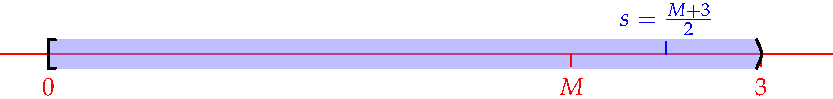
\includegraphics{nomax1}\vspace{-10pt}
	  \end{center}
	  The crux of the argument is to observe that there must be some $s\in S$ which is \emph{larger} than $M$, the natural choice being the average $s:=\frac 12(M+3)$. Now observe that
	  \[
	  	3-s=s-M=\frac 12(3-M)>0
	  \]
	  In particular, $s\in S$ and $s>M$. Since $S$ contains an element larger than $M$, it follows that $M$ cannot be the maximum of $S$. In conclusion, $S$ has no maximum.
	\end{enumerate}
\end{examples}

\footnotetext{%
	$S$ has a maximum means: $\exists M\in S$ such that $\forall s\in S,\ s\le M$. We prove the negation $\forall M\in S, \exists s\in S\text{ such that }s>M$. 
}


\begin{lemm}{}{simpleupperbound}
	\exstart If $M$ is an upper bound for $S$, so is $M+\varepsilon$ for any $\varepsilon\ge 0$.
	%
	\begin{enumerate}\setcounter{enumi}{1}
	  \item If $M=\max S$ exists, then it is unique.
% 	  
% 	  \item $S$ is bounded if and only if it is bounded both above and below. In particular, if $m,M$ are lower/upper bounds, then $S$ is bounded by 
% 	  \[
% 	  	\forall s\in S,\ \nm s\le\max(\nm m,\nm M)
% 	  \]
	\end{enumerate}
\end{lemm}

Try proving these basic facts yourself.
\goodbreak


\begin{example}{}{qsqqrt2nomax}
	In a variation on the previous example, we show that the set
	\[
		S=\Q\cap[0,\sqrt 2)=\{x\in \Q:0\le x<\sqrt 2\}
	\]	
	has no maximum. The approach is similar to before: given a hypothetical maximum $M$, we find some $s\in S$ between $M$ and $\sqrt 2$. The challenge is that we can't use the \emph{average} $\frac 12(M+\sqrt 2)$: this isn't rational (\emph{why?}) and so doesn't lie in $S$!\smallbreak
	
	To fix this, we informally construct a sequence. Define $s_n$ to be $\sqrt 2$ to $n$ decimal places:
	\[
		s_0=1,\quad s_1=1.4=\frac{14}{10},\quad s_2=1.41=\frac{141}{100},\quad s_3=1.414=\frac{1414}{1000},\quad\ldots
	\]
	Since any finite decimal is rational and $0\le s_n<\sqrt 2$, we see that $s_n\in S$. Moreover, $\sqrt 2-s_n\le 10^{-n}$ can be made arbitrarily small by choosing $N$ sufficiently large.\par
	Now suppose $M=\max S$ exists. Since $M\in S$, we have $M<\sqrt 2$. Choose any $N\in\N$ large enough so that $10^{-N}<\sqrt 2-M$ (any integer $N>-\log_{10}(\sqrt 2-M)$ will do!). Certainly $s_N\in S$ and moreover,
	\[
		\sqrt 2 -s_N\le 10^{-N}<\sqrt 2-M\implies M<s_N
	\]
	The purported maximum $M$ is plainly not an upper bound for $S$: contradiction.
	\begin{center}
		\vspace{-5pt}
	  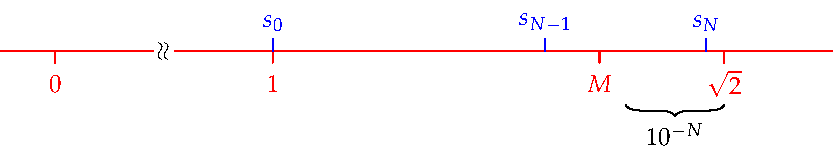
\includegraphics{nomax2}
	\end{center}
\end{example}



\boldsubsubsection{Suprema and Infima}

We generalize the idea of maximum and minimum values to any bounded sets.

\begin{defn}{}{supinf}
	Let $S\subseteq\R$ be non-empty.
	\begin{enumerate}
	  \item If $S$ is bounded above, its \emph{supremum} $\sup S$ is its \emph{least upper bound.} Otherwise said,
		\begin{enumerate}
	  	\item $\sup S$ is an upper bound:\lstsp $\forall s\in S,\ s\le \sup S$,
	  	\item $\sup S$ is the least such:\lstsp if $M$ is an upper bound, then $\sup S\le M$.
		\end{enumerate}
		\item Similarly, if $S$ is bounded below, its \emph{infimum} $\inf S$ is its \emph{greatest lower bound}:
		\begin{enumerate}
	  	\item $\inf S$ is a lower bound:\lstsp $\forall s\in S,\ \inf S\le s$,
	  	\item $\inf S$ is the greatest such:\lstsp if $m$ is a lower bound, then $m\le\inf S$.
		\end{enumerate}
	\end{enumerate}
	\begin{center}
		\vspace{-10pt}
		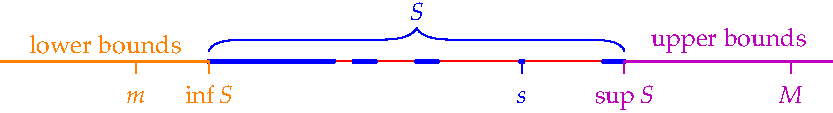
\includegraphics{supinf}
	\end{center}
\end{defn}

\goodbreak




\begin{example}{}{supbasic}
	%\exstart 
	The interval $S=[2,5)$ has $\sup S=5$ and $\inf S=2$ ($=\min S$). We verify these claims: (a), (b) are the properties in the definition.
	%\begin{enumerate}\setcounter{enumi}{1}
	  %\item[]
	  \begin{enumeratea}
			\item Since $s\in S\iff 2\le s<5$, we see that 5 is indeed an upper bound and 2 a lower bound.
			\item We demonstrate the contrapositive. Suppose $M<5$ and define\footnotemark{} $s=\max\{\frac 12(M+5),4\}$. Then $M<s<5$ and $s\in S$. It follows that $M$ is \emph{not} an upper bound for $S$. The least upper bound is therefore $\sup S=5$.\par
			For the infimum: if $m>2$, define $t=\min\{\frac 12(m+2),4\}$ to see that $2<t<m$ and $t\in S$, whence $m$ is not a lower bound.
		\end{enumeratea}
	
		\begin{center}
			\vspace{-5pt}
			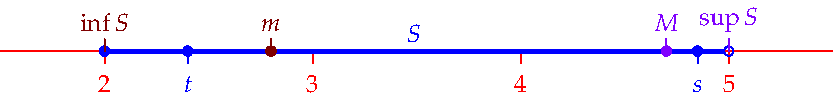
\includegraphics{supinf3}
		\end{center}

% 		\item (Example \ref{ex:qsqqrt2nomax} cont.)\lstsp The set $S=\Q\cap[0,\sqrt 2)$ has $\sup S=\sqrt 2$. We check conditions (a), (b):
% 		\begin{enumerate}
% 			\item Since every element of $S$ is less than $\sqrt 2$, we see that $\sqrt 2$ is an upper bound.
% 			\item If $M<\sqrt 2$ is given, then our previous discussion says there exists some $s_N\in S$ for which $s_N>M$. Plainly $M$ isn't an upper bound.
% 		\end{enumerate}
% 		%In conclusion, $\sqrt 2$ is the smallest upper bound for $S$.
%	\end{enumerate}
\end{example}

\footnotetext{The number 4 is merely an arbitrary element to make sure $s\in S$ in case $M$ were huge and negative!}


\begin{axiom}{Completeness of $\R$}{comp}
	If $S\subseteq\R$ is non-empty and bounded above, then $\sup S$ exists (and is a real number!).
\end{axiom}

It is precisely this property that distinguishes the real numbers from the rationals.\footnote{%
	\label{fn:syntheticR}More formally (the details are too much for us): if $\F$ is an ordered field with $0\neq 1$ and which satisfies the completeness axiom, then $\F$ is isomorphic to the real numbers.%
} Certainly every bounded set $S$ of \emph{rational} numbers has a supremum; the issue is that $\sup S$ \emph{need not be rational}!\smallbreak
By reflecting across zero (Exercise \ref{exs:infexist}), we obtain the same thing for the infimum.

\begin{thm}{Existence of Infima}{infexist}
	If $S\subseteq\R$ non-empty and bounded below, then $\inf S\in\R$ exists.
\end{thm}

\boldinline{A Useful Contrapositive}

Part (b) of the Definition is plainly a biconditional: if $\sup S\le M$, then $M$ is at least as large as an upper bound and is therefore also an upper bound for $S$ (Lemma \ref{lemm:simpleupperbound})! As in Example \ref{ex:supbasic}, one often uses the contrapositive of part (b):

\begin{quote}
	$M<\sup S$ if and only if $M$ is \emph{not} an upper bound for $S$.
\end{quote}

Unpacking this further using the meaning of upper bound (and substituting $x$ for $M$) we recover a useful result that will be used repeatedly.

\begin{lemm}{}{contrasup}
	\exstart Let $S$ be bounded above. Then $\textcolor{Purple}{x<\sup S}\iff\exists \textcolor{blue}{s\in S}$ such that $\textcolor{Purple}{x}<\textcolor{blue}{s}$.
	\begin{enumerate}\setcounter{enumi}{1}
	  \item Let $S$ be bounded below. Then $\textcolor{Red4}{y>\inf S}\iff \exists \textcolor{blue}{t\in S}$ such that $\textcolor{blue}{t}<\textcolor{Red4}{y}$.
	\end{enumerate}
	\begin{center}
		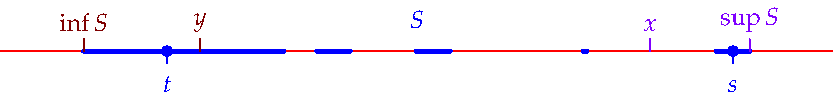
\includegraphics{supinf4}
	\end{center}
\end{lemm}









% \begin{aside}{}{}
% 
% {\bf Aside: A Synthetic Construction of $\R$}\qquad We have only observed that completeness is a \emph{property} of $\R$. It is, in fact, the defining difference between $\R$ and $\Q$. Explicitly:
% 
% \begin{thm}{}{}
% Up to relabeling (isomorphism of fields), there is precisely one set $\R$ which satisfies the following properties:
% \begin{itemize}
% \item $\R$ is an ordered field such that $0\neq 1$ (Axioms \ref{axiom:field} and \ref{axiom:ord})
% \item $\R$ has the completeness property (Axiom \ref{axiom:comp})
% \end{itemize}
% \end{thm}
% 
% \def\SSS{\mathbb{S}}
% The proof is too difficult and far too algebraic for us! To unpack things slightly, one must show that if $(\R,0_\R,1_\R,+_\R,\cdot_\R,\le_\R)$ and $(\SSS,0_\SSS,1_\SSS,+_\SSS,\cdot_\SSS,\le_\SSS)$ are two models satisfying the axioms, then there exists an isomorphism $\phi:\R\to\SSS$: that is,
% \begin{enumerate}
%   \item $\phi$ is bijective
%   %\item $\phi(0_\R)=0_\SSS$ and $\phi(1_\R)=1_\SSS$
%   \item $\phi(x+_\R y)=\phi(x)+_\SSS\phi(y)$ and $\phi(x\cdot_\R y)=\phi(x)\cdot_\SSS\phi(y)$ for all $x,y\in\R$
%   \item $x\le_\R y\iff \phi(x)\le_\SSS\phi(y)$
% \end{enumerate}
% 
% This approach will likely only satisfy you if you are addicted to abstract algebra!
% \end{aside}

\goodbreak


\begin{examples}{}{}
	We state the following without proof or calculation. You should be able to justify everything using the definition, or by mirroring Example \ref{ex:supbasic}.
	\begin{enumerate}
		\item A bounded set has many possible bounds, but only one supremum or infimum.
		\item If $S$ has a maximum, then $\max S=\sup S$. Similarly, if a minimum exists, then $\min S=\inf S$.
		%\item The supremum and infimum exist even when a maximum and minimum do not. For instance, $S=(-1,4)$ has $\sup S=4$; the set has no maximum since $\sup S=4\not\in S$. Similarly, $S$ has no minimum and $\inf S=-1\not\in S$.
		\item (Example \ref{ex:qsqqrt2nomax})\lstsp $S=\Q\cap[0,\sqrt 2)$ has $\sup S=\sqrt 2$: this is a set of rational numbers whose supremum is not rational.
		\item $S=\Q\cap (\pi,4)$ has $\sup S=4$, $\inf S=\pi$, and no maximum nor minimum.
		\item $S=\{\frac 1n:n\in\N\}=\{\ldots,\frac 14,\frac 13,\frac 12,1\}$ has $\sup S=\max S=1$, $\inf S=0$, and no minimum.
		\item $S=\bigcup\limits_{n=1}^\infty [n,n+\frac 12)=[1,1.5)\cup[2,2.5)\cup[3,3.5)\cup\cdots$ has $\inf S=1$. It is not bounded above.
		\item $S=\bigcap\limits_{n=1}^\infty [\frac 1n,1+\frac 1n)$ has $\inf S=1=\sup S$ since $S=\{1\}$.
	\end{enumerate}
\end{examples}



\boldsubsubsection{The Archimedean Property and the Density of the Rationals}

We finish this section by discussing a crucial property related to completeness, and of the distribution of the rational numbers among the reals.

\begin{thm}{Archimedean Property}{archprop}
	If $b>0$ is a real number, then $\exists n\in\N$ such that $n>b$.\smallbreak
	More generally: $a,b>0\implies \exists n\in\N$ such that $an>b$.
\end{thm}

We assume nothing about $\R$ except that is an ordered field satisfying the completeness axiom and where $0\neq 1$ (footnote \ref{fn:syntheticR}). The natural numbers in this context are \emph{defined} as the subset
\[
	\N=\{1,1+1,1+1+1,\ldots\}\subseteq\R
\]
and Peano's axioms are a \emph{theorem.} %In the next section we'll briefly think about how the Archimidean property is essentially trivial if one has an \emph{explicit} construction of $\R$ built upon $\N$ and $\Q$.

\begin{proof}
	Suppose the result were false. Then $\exists b>0$ such that $n\le b$ for all $n\in\N$; that is, $\N$ is bounded above! By completeness, $\sup\N$ exists, and we trivially see that
	\[
		0<1\implies \sup\N<\sup\N+1\implies \sup\N-1<\sup\N
	\]
	By Lemma \ref{lemm:contrasup}, $\exists n\in\N$ such that $n>\sup\N-1$. But then $\sup\N<n+1$ which is clearly a natural number! Thus $\sup\N$ is not an upper bound for $\N$: contradiction.\smallbreak
	For the more general statement, simply replace $b$ with $\frac ba$.
\end{proof}

The use of completeness is \emph{necessary}: there exist \href{https://en.wikipedia.org/wiki/Non-Archimedean_ordered_field}{non-Archimedean ordered fields!}\medbreak

\begin{example*}{\ref{ex:qsqqrt2nomax}, cont.}
	The Archimedean property is precisely what is needed to justify the existence of an integer $N>-\log_{10}(\sqrt 2-M)$.
\end{example*}


\goodbreak


\begin{cor}{Density of $\Q$ in $\R$}{qdense}
	Between any two real numbers, there exists a rational number.
\end{cor}

The idea is hopefully straightforward: given $a<b$, \textcolor{blue}{stretch} the interval by an integer factor $n$ until it contains an integer $m$, before \textcolor{Purple}{dividing} by $n$ to obtain $a<\frac mn<b$. We use the Archimedean property to establish the existence of the scale factors $m,n$.

\begin{proof}
	Suppose WLOG that $0\le a<b$, and apply the Archimedean property to $\frac 1{b-a}>0$:
	\[
		\exists n\in\N\ \text{such that}\ n>\tfrac 1{b-a}
	\]
	A second application (or trivially if $a=0$) says $\exists k\in\N$ such that $\textcolor{Green}{k}>\textcolor{blue}{an}$. Now consider the set
	\[
		J:=\{j\in\N:\textcolor{blue}{an}<\textcolor{Green}{j}
		\le\textcolor{Green}{k}\}
	\]
	and define $\textcolor{Green}{m}=\min J$: this exists since $J$ is a finite non-empty set of natural numbers.\footnotemark{}
	\begin{center}
		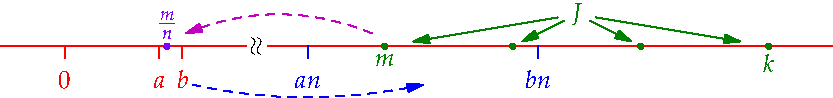
\includegraphics{density}
	\end{center}
	Clearly $\textcolor{Green}{m}>\textcolor{blue}{an}>m-1$, since $\textcolor{Green}{m}=\min J$. But then $\textcolor{Green}{m}\le an+1<\textcolor{blue}{bn}$. We conclude that
	\[
		\textcolor{blue}{an}<\textcolor{Green}{m}<\textcolor{blue}{bn}
		\implies a<\textcolor{purple}{\frac mn}<b\tag*{\qedhere}
	\]
\end{proof}

\footnotetext{%
	This part of the argument is necessary since, in this context, we haven't established the well-ordering property of $\N$ (essentially Peano's fifth axiom).%
}

By iterating this result we see that any interval $(a,b)$ contains \emph{infinitely many} rational numbers. It can moreover be established that the irrational numbers are also dense in $\R$ (Exercise \ref{exs:irrdense}).

%\bigbreak



\begin{exercises}{}{}
	\emph{Key concepts:\quad Suprema,\quad Completeness (distinguishes $\R$),\quad Contrapositive criterion,}
	\begin{quote}
		\emph{Archimedean property/Density of $\Q\subset\R$}
	\end{quote}
	
	\begin{enumerate}
	  \item Decide whether each set is bounded above and/or below. If so, state its supremum and/or infimum (no working is required).
	  \begin{enumerate}
	    \item \makebox[130pt][l]{$(0,1)$\hfill (b)} \makebox[170pt][l]{\ $\{2,7\}$\hfill (c)} \ $\{0\}$
	    \setcounter{enumii}{3}
	    \item \makebox[130pt][l]{$\bigcup\limits_{n=1}^\infty[2n,2n+1]$\hfill (e)} \makebox[170pt][l]{\ $\left\{1-\frac 1{3^n}:n\in\N\right\}$\hfill (f)} \ $\{r\in\Q:r^2<2\}$
	    \setcounter{enumii}{6}
	    \item \makebox[130pt][l]{$\bigcup\limits_{n=1}^\infty\left(1-\frac 1n,1+\frac 1n\right)$\hfill (h)} \makebox[170pt][l]{\ $\{\frac 1n:n\in\N$ and $n$ is prime$\}$\hfill (i)} \ $\{\cos(\frac{n\pi}3):n\in\N\}$
  \end{enumerate}

  
  	\item Modelling Example \ref{ex:qsqqrt2nomax}, \emph{sketch} an argument that $S=\Q\cap (\pi,4]$ has no minimum.\par
  	(\emph{Hint: let $s_n$ be $\pi$ rounded \underline{up} to $n$ decimal places})
  
  
  	\goodbreak
  
  
		\item %(6)
		Let $S$ be a non-empty, bounded subset of $\R$.
  	\begin{enumerate}
		  \item Prove that $\inf S\le \sup S$. %(Proof should be short\ldots)
		  \item What can you say about $S$ if $\inf S=\sup S$?
  	\end{enumerate}
  
  
  	\goodbreak
  
  
	  \item %(7) 
	  Let $S$ and $T$ be non-empty subsets of $\R$ with the property that $s\le t$ for all $s\in S$ and $t\in T$.
	  \begin{enumerate}
		  \item Prove that $S$ is bounded above and $T$ bounded below.
		  \item Prove that $\sup S\le \inf T$.
		  \item Give an example of such sets $S,T$ where $S\cap T$ is non-empty.
		  \item Give an example of such sets $S,T$ where $S\cap T$ is empty, and $\sup S=\inf T$.
	  \end{enumerate}
  
  
	  \item %(9)
	  Prove that if $a>0$ then there exists $n\in\N$ such that $\frac 1n<a<n$.
	  
	
	  \item%(12) 
	  \label{exs:irrdense} Let $\II=\R\setminus\Q$ be the set of \emph{irrational} numbers. Given real numbers $a<b$, prove that there exists $x\in\II$ such that $a<x<b$.\par
	  (\emph{Hint: First show $\{r+\sqrt 2:r\in\Q\}\subseteq\II$})
  

  	\item %(14)
  	Let $A, B$ be non-empty bounded subsets of $\R$, and let $S$ be the set of all sums
  	\[
  		S:=\{a+b:a\in A,b\in B\}
  	\]
	  \begin{enumerate}
		  \item Prove that $\sup S=\sup A+\sup B$.
		  \item Prove that $\inf S=\inf A+\inf B$.
	  \end{enumerate}
  

  	\item%(16)
  	Show that $\sup\{r\in \Q:r<a\}=a$ for each $a\in\R$.
  
  
  	\item\label{exs:infexist} We prove Theorem \ref{thm:infexist} on the existence of the infimum.\smallbreak
	  Let $S\subseteq\R$ be non-empty and let $m$ be a lower bound for $S$. Define $T=\{t\in\R:-t\in S\}$ by \textcolor{red}{reflecting} $S$ across zero.
		\begin{center}
			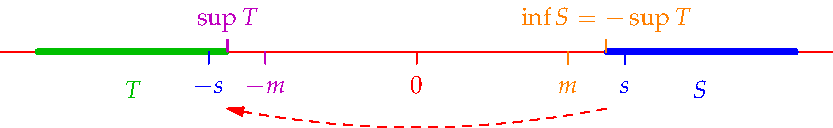
\includegraphics{infexist2}
		\end{center}
		\begin{enumerate}
		  \item Prove that $-m$ is an upper bound for $T$.
			\item By completeness (Axiom \ref{axiom:comp}), $\sup T$ exists. Prove that $\inf S=-\sup T$ by verifying Definition \ref{defn:supinf} parts 2(a) and (b).
		\end{enumerate}
  
	\end{enumerate}
\end{exercises}


\clearpage


\subsection[The Symbols +/- Infinity]{The Symbols $\pm\infty$}

Thus far the only subsets of the real numbers that have a supremum are those which are \emph{non-empty} and \emph{bounded above.} In this very short section, we introduce the $\infty$-symbol to provide all subsets of the real numbers with both a supremum and an infimum.

\begin{defn}{}{}
	Let $S\subseteq\R$ be any subset. If $S$ is bounded above/below, then $\sup S$/$\inf S$ are as in Definition \ref{defn:supinf}. Otherwise:
	\begin{enumerate}
	  \item We write $\sup S=\infty$ if $S$ is \emph{unbounded above}, that is
	  \[
	  	\forall x\in \R, \exists s\in S\text{ such that }s>x
	  \]
	  \item We write $\inf S=-\infty$ if $S$ is \emph{unbounded below},
	  \[
	  	\forall y\in \R, \exists t\in S\text{ such that }t<y
	  \]
	  \item By convention, $\sup\emptyset:=-\infty$ and $\inf\emptyset:=\infty$, though these will rarely be of use to us.
	\end{enumerate}
\end{defn}

The symbols $\pm\infty$ have \emph{no other meaning} (as yet); in particular, they are \emph{not numbers}. If one is willing to abuse notation and write $x<\infty$ and $y>-\infty$ for any real numbers $x,y$, then the conclusions of Lemma \ref{lemm:contrasup} are precisely statements 1 \& 2 above!


\begin{examples}{}{}
	\exstart $\sup\R=\sup\Q=\sup\Z=\sup\N=\infty$, since all are unbounded above. We also have $\inf\R=\inf\Q=\inf\Z=-\infty$ (recall that $\inf\N=\min\N=1$).
	\begin{enumerate}\setcounter{enumi}{1}
	  \item If $a<b$, then \emph{any} interval $[a,b]$, $(a,b)$, $[a,b)$ or $(a,b]$ has supremum $b$ and infimum $a$, even if one end is infinite. For example,
		\[
			S=(7,\infty)=\{x\in\R:x>7\}
		\]
		has $\sup S=\infty$ and $\inf S=7$.
		\item Let $S=\{x\in\R:x^3-4x<0\}$. With a little factorization, we see that
		\[
			x^3-4x=x(x-2)(x+2)<0\iff x<-2\text{ or }0<x<2
		\]
		It follows that $S=(-\infty,-2)\cup(0,2)$, from which $\sup S=2$ and $\inf S=-\infty$.  
	\end{enumerate}
\end{examples}


\begin{exercises}{}{}
	\emph{Key concepts:\quad $\pm\infty$ are shorthands for \textbf{unboundedness}: they are \textbf{not numbers}!}
	
	\begin{enumerate}
	  \item Give the infimum and supremum of each of the following sets:
	  \begin{enumerate}
	    \item \makebox[160pt][l]{$\{x\in\R:x<0\}$ \hfill (b)} \ $\{x\in\R:x^3\le 8\}$
	    \setcounter{enumii}{2}
	    \item \makebox[160pt][l]{$\{x^2:x\in\R\}$ \hfill (d)} \ $\{x\in\R:x^2<8\}$
	  \end{enumerate}
	  
	
	  \item%(4)
	  Let $S\subseteq\R$ be non-empty, and let $-S=\{-s:s\in S\}$. Prove that $\inf S=-\sup(-S)$.
	
	
	  \item%(6)
	  Let $S,T\subseteq\R$ be non-empty such that $S\subseteq T$. Prove that $\inf T\le \inf S\le \sup S\le\sup T$.
	  
	  \item If $\sup S<\inf S$, what can you say about $S$?
	  
	\end{enumerate}
\end{exercises}


\clearpage


\subsection[A Development of R]{A Development of $\R$ (non-examinable)}\label{sec:dedekind}

The comment in footnote \ref{fn:syntheticR} constitutes a \emph{synthetic} definition of the real numbers: there is essentially just one set with the required properties. While this might satisfy an algebra-addict, it is nice to be able to provide an explicit construction. The following approach uses so-called \emph{Dedekind cuts.}\medbreak

First one defines $\N$, $\Z$ and $\Q$. Use Peano's axioms and proceed as in sections \ref{sec:natural} and \ref{sec:Q}. The operations $+,\cdot$ and $\le$ are defined, first on $\N$ and then for $\Z$ and $\Q$ building on these concepts for the integers.

\begin{defn}{}{dedekind}
	A \emph{Dedekind cut} $\alpha^*$ is a non-empty proper subset of $\Q$ with the properties:
	\begin{enumerate}
  	\item (Closed downwards)\lstsp If $r\in\alpha^*$ and $s\in\Q$ with $s<r$, then $s\in\alpha^*$.
  	%\item $\alpha^*$ is bounded above.
  	\item (No maximum)\lstsp If $M$ is an upper bound for $\alpha^*$, then $M\not\in\alpha^*$.
	\end{enumerate}
	Define $\R$ to be the set of all Dedekind cuts!
\end{defn}

The rough idea is that a real number $\alpha$ corresponds to the Dedekind cut $\alpha^*$ of all \emph{rational numbers less than $\alpha$.}

\begin{examples}{}{}
	\exstart For any \emph{rational number} $r$, the corresponding \emph{real number} is the Dedekind cut
	\[
		r^*=\{x\in\Q:x<r\}
	\]
	\begin{enumerate}\setcounter{enumi}{1}
	  \item[]For instance $4^*=\{x\in\Q:x<4\}$ is the Dedekind cut definition of the  \emph{real number} 4.
	  \item It is a little trickier to explicitly define cuts corresponding to irrational numbers, though some are relatively straightforward. For instance the real number $\sqrt 2$ would be the set
		\[
			{\sqrt 2\,}^*=\{x\in\Q:x<0\text{ or }x^2<2\}
		\]
	\end{enumerate}
\end{examples}

It remains to \emph{prove} that the set of Dedekind cuts satisfies the axioms of a complete ordered field. The full details are too much, so here is a rough overview.
\begin{itemize}
  \item Define the ordering of Dedekind cuts via
	\[
		\alpha^*\le\beta^*\iff\alpha^*\subseteq\beta^*
	\]
	One can now prove axioms O1--O3 and that the ordering corresponds to that of $\Q$.
	\item Define addition of cuts via
	\[
		\alpha^*+\beta^*:=\{a+b:a\in\alpha^*,b\in\beta^*\}
	\]
	This suffices to prove the addition axioms and O4: a careful definition of $-\alpha^*$ is required.
	\item Multiplication is horrible: if $\alpha^*,\beta^*\ge 0^*$ then
	\[
		\alpha^*\beta^*:=\{ab:a\ge 0,a\in \alpha^*,b\ge 0,b\in \beta^*\}\cup\{q\in\Q:q<0\}
	\]
	which may be carefully extended to cover situations when $\alpha^*$ or $\beta^*<0^*$. Once this has been done, one can then prove the multiplication axioms, the final order axiom O5, and the distributive axiom.
	\item The completeness axiom must also be verified, though it comes almost for free! If $A\subseteq\R$ (a set of Dedekind cuts), then the supremum of $A$ is simply
	\[
		\sup A=\bigcup\limits_{\alpha^*\in A}\alpha^*
	\]
	Think about it\ldots
\end{itemize}

An alternative approach to $\R$ using sequences of rational numbers will be given later.


\begin{exercises}{}{}
	\emph{Key concepts:\quad $\R$ is unnatural and difficult to construct in a logical manner}

	\begin{enumerate}
	  \item Show that if $\alpha^*,\beta^*$ are Dedekind cuts, then so is
  	\[
  		\alpha^*+\beta^*=\{r_1+r_2:r_1\in\alpha^*,r_2\in\beta^*\}
  	\]
	  
	  
	  \item %(4)
	  Let $\alpha^*,\beta^*$ be Dedekind cuts and define the `product':
	  \[
	  	\alpha^*\cdot\beta^*=\{r_1r_2:r_1\in\alpha^*,r_2\in\beta^*\}
	  \]
	  \begin{enumerate}
	  	\item Calculate some `products' using the cuts $0^*,1^*$ and $(-1)^*$.
	  	\item Discuss why this `product' is unsatisfactory for defining multiplication in $\R$.
	  \end{enumerate}
	  
	  
	  \item We verify the Archimedean property (Theorem \ref{thm:archprop}) using the Dedekind cut definition of $\R$ (it is somewhat easier since the unboundedness of $\N$ and $\Q$ are baked in).
	  \begin{enumerate}
	    \item Explain why every cut $\beta^*$ is bounded above by some rational number.\par
	    (\emph{Hint: if $\beta^*$ satisfies Definition \ref{defn:dedekind} parts 1 \& 2 but is unbounded above, then what is it?})
	    \item If $\beta^*>0^*$ is a positive cut bounded above by $\frac pq$ with $p,q\in\N$, show that $n:=p+1$ corresponds to a cut for which $n^*>\beta^*$.
		\end{enumerate}
	\end{enumerate}
\end{exercises}